

\Idit{Todo: update API to include brc, bwc, br, wc, and example combinations, some of which are supported.}

We support a restricted set of local transactions, focusing on short ones that
frequently occur in production. Recall that short transactions benefit most from
our optimizations since for them, the overhead of performing centralized coordination once or twice
per transaction is significant.

There are two distinctive characteristics of local transactions. First, they
must access a single region. Second, in contrast to regular transactions, they
cannot dynamically evolve, but rather must be provided in their entirety with a
single API call: 
local transactions forgo the standard API including begin and commit operations,
and instead invoke a single function for executing the entire transaction. The
new API functions for local transactions are prefixed with \code{LTX\_}. 

The simplest examples are singleton transactions, i.e., transactions that perform a single
read operation via \code{LTX\_read(key)} or a single update via \code{LTX\_write(key, value)}. 
The latter creates a new version for key that exceeds all existing ones.

A more elaborate example is a multi-read-single-write API, \code{LTX\_MRSW(\wkey, \rkeys, f)}, 
which atomically reads values associated  with a list of \rkeys and updates the value associated with
\wkey according to some function f of the read values. Note that this API
is applicable only in case \wkey and all \rkeys reside in the same region. In case
they do not, the call fails, and the transaction may be restarted as a regular
transaction.

The semantics for ordering local transactions relative to regular ones are
weaker than SI in that they do not guarantee real-time order over all regular
and local transactions together. Specifically, a regular transaction overlapping
two local transactions that access different regions may observe the updates of
the second and miss an update by the first. For example, assume objects x and y
are managed in two different regions, then real-time order can be violated as
illustrated in Figure~\ref{fig:ltx-rt} (ignore the skip operations for now; they will be explained in the next section).

\begin{figure}[h]
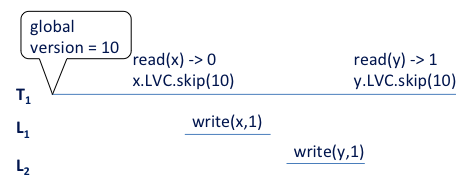
\includegraphics[width=\columnwidth]{LTX-RT}
\caption{Possible violation of real-time order among local transactions in different regions. Global transaction $T_1$
reads $x$ before it is updated by local transaction $L_1$ and reads $y$ after it is updated by local transaction $L_2$ even 
though $L_2$ occurs after $L_1$. $T1$'s global version is $10$, and its skips the local version clocks of the regions holding $x$ and $y$ to $10$ when reading from them.}
\label{fig:ltx-rt}
\end{figure}

The system still enforces a total order on all committed transactions, so that
\begin{enumerate}
    \setlength{\itemsep}{0pt}
    \setlength{\parskip}{0pt}
    \setlength{\parsep}{2pt}  
\item
regular transactions (though not local ones) are ordered according to their commit times;
\item
each transaction's read operations see a consistent snapshot of the database reflecting 
a sequence of transactions that includes all those committed prior to
its start time plus any number of concurrent local transactions; and 
\item
 a transaction commits only if none of the items it updates has been modified since that snapshot.
 \end{enumerate}

\idit{Todo: add a note about causality being preserved because re-ordering can only occur across regions.}
